\documentclass{article}[10 pt,landscape]
\usepackage{graphicx, graphics}
\usepackage{lscape}

\begin{document}
\newcommand{\bs}{\backslash}

\title{Roulette}

You are to construct a digital circuit that plays a game of
roulette, allows betting and keeps track of total earnings.
The roulette wheel has 8 slots, labeled $1 \ldots 8$.  The player
can play one of the numbers straight or play even or odd.
The player starts with \$10.
The layout of the machine is shown in Figure~\ref{fig:Roulette}.
\begin{figure}[ht]
    \center{\scalebox{0.5}{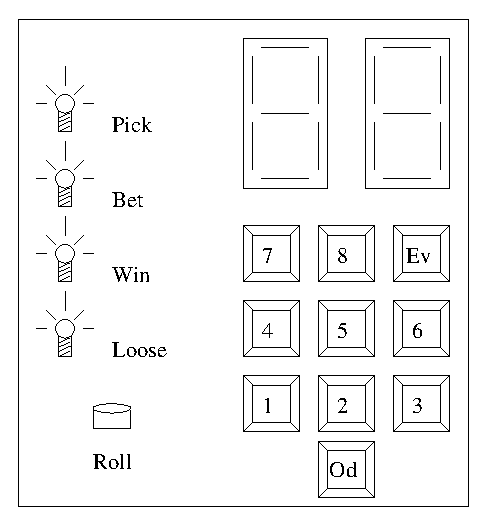
\includegraphics{./Prob8-17}}}
    \caption{The layout of the roulette playing machine.
        The two 7 segment displays at the top are used for a variety
    of purposes.}
    \label{fig:Roulette}
\end{figure}

The sequence of events is as follows:
\begin{enumerate}
    \item    The circuit lights up the PICK LED.
        The player enters their guess; a number between 1-8, even or odd.
        While holding down their guess they press the roll button.
    \item    The circuit displays the picked number in the left most
        7 segment display.  The circuit lights up the BET LED.
        The player enters a one digit bet between 1 to 8.  While holding
        down their bet they press the roll button.
    \item     The circuit displays the bet on the rightmost 7-segment
        display.
        The player pushes and holds down the roll button.
        The circuit increments a mod 8 counter while the roll
        button is depressed. It would be nice to display the
        current count value on right 7-seven segment display.
        Since the clock cycle is on the order of milliseconds,
        then the user would not be able to anticipate the roll.
    \item    The player releases the roll button.  The final roll
        is displayed on the rightmost 7-segment display.
        The circuit stops incrementing the counter and checks
        to see if the final value matches the players guess.
        If the match is correct then light the WIN LED and
        increment the players earnings.  If the match is incorrect
        then light the LOOSE LED and decrement the players
        earnings.
    \item    The play hits the roll button to clear the roll information
        from the 7-segment displays.
    \item    The circuit displays the players earnings on the 7-segment
        display.
    \item    When the user pushes the roll button then goto step 1.
\end{enumerate}

Set reasonable bounds on the maximum winnings.  Values may be displayed
in hexadecimal (you may assume that you have a hex to 7-segment display
converter at your disposal).
\\
\\

{\bf Algorthm}
{\small
    \\
    1. cash = 10; \\
    2. LeftSeven = blank;     \\
    3. RightSeven = cash;     \\
    4. while(cash != 0) {     \\
        5.     LEDarray = 1 0 0 0;    // Pick Bet Win Loose     \\
        6.     while(ROLL == 0);     \\
        7.     guess = Datain;     \\
        8.     while(ROLL == 1);     \\
        9.          \\
        10.     LEDarray = 0 1 0 0;    // Pick Bet Win Loose     \\
        11.     LeftSeven = guess;     \\
        12.     RightSeven = blank;     \\
        13.     while(ROLL == 0);     \\
        14.     bet = Datain;     \\
        15.     while(ROLL == 1);     \\
        16.          \\
        17.     LEDarray = 0 0 0 0;    // Pick Bet Win Loose     \\
        18.     RightSeven = bet;     \\
        19.     while(ROLL == 0);     \\
        20.     while(ROLL == 1) count = count + 1;     \\
        21.      \\
        22.     RightSeven = count;     \\
        23.     if (count == guess) {     \\
            24.         cash = cash + (bet *4);     \\
            25.         LEDarray = 0 0 1 0;    // Pick Bet Win Loose     \\
        26.     } else {     \\
            27.         cash = cash - bet;     \\
            28.         LEDarray = 0 0 0 1;    // Pick Bet Win Loose     \\
        29.     }     \\
        30.     while(ROLL == 0);     \\
        31.     while(ROLL == 1);     \\
        32.     RightSeven = cash;     \\
        33.      \\
    34. }         \\
    35. LEDarray = 0 0 0 1;    // The user is out of money     \\
    36. while(1);        // Halt the machine     \\
}

\begin{landscape}
    {\bf Datapath and Control}
    \begin{figure}[ht]
        \center{\scalebox{0.7}{\includegraphics{./Sol8-16-blank}}}
    \end{figure}

    \pagebreak
    {\bf Control Word}

    {\normalsize
        \begin{tabular}{l|l|l|l|l|l|l|l|l|l|l}
            State &  counter& guess  & bet    & cmux      & bmux     & cash   & add/sub & ledmux    & rmux
            & lmux \\ \hline
            & 00 hold & 0 hold & 0 hold & 0 \$10    & 0 bet    & 0 hold & 0 add  & 00 (pick) &00 cash &00
            cash  \\ \hline
            & 01 load & 0 load & 1 load & 1 add/sub & 1 bet<<2 & 1 load & 1 sub  & 01 (bet ) &01 bet  &01
            guess \\ \hline
            & 10 up   &        &        &            &          &        &        & 10 (win ) &10 count&10
            blank \\ \hline
            &         &        &        &            &          &        &        & 11 (loose)&11 blank&
            \\ \hline
            &         &        &        &            &          &        &        &          &         &   \\ \hline
            init  &       &       &       &           &         &       &       &        &       & \\ \hline
            wg1   &       &       &       &           &         &       &       &        &       & \\ \hline
            guess &       &       &       &           &         &       &       &        &       & \\ \hline
            wg2   &       &       &       &           &         &       &       &        &       & \\ \hline
            wb1   &       &       &       &           &         &       &       &        &       & \\ \hline
            bet   &       &       &       &           &         &       &       &        &       & \\ \hline
            wb2   &       &       &       &           &         &       &       &        &       & \\ \hline
            wr1   &       &       &       &           &         &       &       &        &       & \\ \hline
            spin  &       &       &       &           &         &       &       &        &       & \\ \hline
            load 1&       &       &       &           &         &       &       &        &       & \\ \hline
            comp  &       &       &       &           &         &       &       &        &       & \\ \hline
            win   &       &       &       &           &         &       &       &        &       & \\ \hline
            add   &       &       &       &           &         &       &       &        &       & \\ \hline
            loose &       &       &       &           &         &       &       &        &       & \\ \hline
            sub &       &       &       &           &         &       &       &        &       & \\ \hline
            wn    &       &       &       &           &         &       &       &        &       & \\
        \end{tabular}
    }
\end{landscape}

\end{document}
